%% PNAStmpl.tex
%% Template file to use for PNAS articles prepared in LaTeX
%% Version: Apr 14, 2008


%%%%%%%%%%%%%%%%%%%%%%%%%%%%%%
%% BASIC CLASS FILE
%% PNAStwo for two column articles is called by default.
%% Uncomment PNASone for single column articles. One column class
%% and style files are available upon request from pnas@nas.edu.
%% (uncomment means get rid of the '%' in front of the command)

%\documentclass{pnasone}
\documentclass{pnastwo}

%%%%%%%%%%%%%%%%%%%%%%%%%%%%%%
%% Changing position of text on physical page:
%% Since not all printers position
%% the printed page in the same place on the physical page,
%% you can change the position yourself here, if you need to:

% \advance\voffset -.5in % Minus dimension will raise the printed page on the
                         %  physical page; positive dimension will lower it.

%% You may set the dimension to the size that you need.

%%%%%%%%%%%%%%%%%%%%%%%%%%%%%%
%% OPTIONAL GRAPHICS STYLE FILE

%% Requires graphics style file (graphicx.sty), used for inserting
%% .eps files into LaTeX articles.
%% Note that inclusion of .eps files is for your reference only;
%% when submitting to PNAS please submit figures separately.

%% Type into the square brackets the name of the driver program
%% that you are using. If you don't know, try dvips, which is the
%% most common PC driver, or textures for the Mac. These are the options:

% [dvips], [xdvi], [dvipdf], [dvipdfm], [dvipdfmx], [pdftex], [dvipsone],
% [dviwindo], [emtex], [dviwin], [pctexps], [pctexwin], [pctexhp], [pctex32],
% [truetex], [tcidvi], [vtex], [oztex], [textures], [xetex]

%\usepackage[dvips]{graphicx}

%%%%%%%%%%%%%%%%%%%%%%%%%%%%%%
%% OPTIONAL POSTSCRIPT FONT FILES

%% PostScript font files: You may need to edit the PNASoneF.sty
%% or PNAStwoF.sty file to make the font names match those on your system.
%% Alternatively, you can leave the font style file commands commented out
%% and typeset your article using the default Computer Modern
%% fonts (recommended). If accepted, your article will be typeset
%% at PNAS using PostScript fonts.

% Choose PNASoneF for one column; PNAStwoF for two column:
%\usepackage{PNASoneF}
\usepackage{PNAStwoF}

%%%%%%%%%%%%%%%%%%%%%%%%%%%%%%
%% ADDITIONAL OPTIONAL STYLE FILES

%% The AMS math files are commonly used to gain access to useful features
%% like extended math fonts and math commands.

\usepackage{amssymb,amsfonts,amsmath}

\graphicspath{ {paper_figures2/} }

%\usepackage{tikz}

%%%%%%%%%%%%%%%%%%%%%%%%%%%%%%
%% OPTIONAL MACRO FILES
%% Insert self-defined macros here.
%% \newcommand definitions are recommended; \def definitions are supported

%\newcommand{\mfrac}[2]{\frac{\displaystyle #1}{\displaystyle #2}}
%\def\s{\sigma}


\newcommand{\SI}[0]{{\it SI Materials and Methods}}
\newcommand{\fig}[0]{Fig.}


\makeatletter
\newcommand{\customlabel}[2]{%
\protected@write \@auxout {}{\string \newlabel {#1}{{#2}{}}}}
\makeatother

\customlabel{fig:DV_view}{S1}
\customlabel{fig:membrane_curve}{S2}
\customlabel{fig:raw_data3}{S3}
\customlabel{fig:1d_example}{S4}
\customlabel{fig:spheres}{S5}
\customlabel{fig:eigenvalues}{S6}
\customlabel{fig:PCA_data1}{S7}
\customlabel{fig:PCA_data2}{S8}

%%%%%%%%%%%%%%%%%%%%%%%%%%%%%%
%% Don't type in anything in the following section:
%%%%%%%%%%%%
%% For PNAS Only:
\contributor{Submitted to Proceedings
of the National Academy of Sciences of the United States of America}
\url{www.pnas.org/cgi/doi/10.1073/pnas.0709640104}
\copyrightyear{2008}
\issuedate{Issue Date}
\volume{Volume}
\issuenumber{Issue Number}
%%%%%%%%%%%%

\begin{document}

%%%%%%%%%%%%%%%%%%%%%%%%%%%%%%


%% For titles, only capitalize the first letter
%% \title{Almost sharp fronts for the surface quasi-geostrophic equation}

\title{Temporal ordering and registration of images in studies of developmental dynamics}

%% Enter authors via the \author command.
%% Use \affil to define affiliations.
%% (Leave no spaces between author name and \affil command)

%% Note that the \thanks{} command has been disabled in favor of
%% a generic, reserved space for PNAS publication footnotes.

%% \author{<author name>
%% \affil{<number>}{<Institution>}} One number for each institution.
%% The same number should be used for authors that
%% are affiliated with the same institution, after the first time
%% only the number is needed, ie, \affil{number}{text}, \affil{number}{}
%% Then, before last author ...
%% \and
%% \author{<author name>
%% \affil{<number>}{}}

%% For example, assuming Garcia and Sonnery are both affiliated with
%% Universidad de Murcia:
%% \author{Roberta Graff\affil{1}{University of Cambridge, Cambridge,
%% United Kingdom},
%% Javier de Ruiz Garcia\affil{2}{Universidad de Murcia, Bioquimica y Biologia
%% Molecular, Murcia, Spain}, \and Franklin Sonnery\affil{2}{}}

\author{Carmeline~J.~Dsilva\affil{1}{Department of Chemical and Biological Engineering, Princeton University, Princeton, New Jersey, USA},
Bomyi~Lim\affil{1}{},
Thomas~J.~Levario\affil{2}{School of Chemical and Biomolecular Engineering, Georgia Institute of Technology, Atlanta, Georgia, USA},
Hang~Lu\affil{2}{},
Amit~Singer\affil{3}{Department of Mathematics, Princeton University, Princeton, New Jersey, USA} \affil{4}{Program in Applied and Computational Mathematics, Princeton University, Princeton, New Jersey, USA},
Stanislav~Y.~Shvartsman\affil{1}{} \affil{5}{Lewis-Sigler Institute for Integrative Genomics, Princeton University, Princeton, New Jersey, USA},
\and
Ioannis~G.~Kevrekidis\affil{1}{} \affil{4}{Program in Applied and Computational Mathematics, Princeton University, Princeton, New Jersey, USA}}

\contributor{Submitted to Proceedings of the National Academy of Sciences
of the United States of America}

\significancetext{
Imaging studies are commonly used to study developmental dynamics in multiple organisms. 
%
When many samples are involved in a single study,
one of the first steps in data analysis involves registration and temporal ordering of images. 
%
Here we show that both of these tasks can be automated and combined in a single step using recent advances in data mining. 
%
To illustrate this approach, we temporally order and register several data sets collected in  studies of cell signaling in the early fruit fly embryo.}

%% The \maketitle command is necessary to build the title page.
\maketitle

%%%%%%%%%%%%%%%%%%%%%%%%%%%%%%%%%%%%%%%%%%%%%%%%%%%%%%%%%%%%%%%%
\begin{article}

\begin{abstract}

Imaging studies provide unique insights into the dynamics of developmental processes. 
%
Often, data is collected across many samples in several experiments, and the first task is to organize the data for further analysis.
%
This includes spatially registering images of different biological samples, and well as
temporally ordering the data to reconstruct representative developmental dynamics.
%
When such data sets are large, noisy, and/or if the developmental changes are subtle, these tasks can be difficult to perform manually.
%
We present an automated approach to simultaneously register and temporally order imaging data sets.
%
The approach is based on vector diffusion maps, a broadly applicable manifold learning technique that does not require {\it a priori} knowledge of image features or a parametric model of the developmental dynamics.
%
We validate this approach using a live imaging data set where both the correct rotational orientation and temporal order are known, as well as use these methods to extract a developmental trajectory from a data set of fixed images collected to study dorsoventral patterning of the {\it Drosophila} embryo.

\end{abstract}

%% When adding keywords, separate each term with a straight line: |
\keywords{temporal ordering | image registration | vector diffusion maps}

%\section{Significance}

%\vspace{0.5cm}

%% Optional for entering abbreviations, separate the abbreviation from
%% its definition with a comma, separate each pair with a semicolon:
%% for example:
%% \abbreviations{SAM, self-assembled monolayer; OTS,
%% octadecyltrichlorosilane}

% \abbreviations{}

%% The first letter of the article should be drop cap: \dropcap{}
%\dropcap{I}n this article we study the evolution of ''almost-sharp'' fronts

%% Enter the text of your article beginning here and ending before
%% \begin{acknowledgements}
%% Section head commands for your reference:
%% \section{}
%% \subsection{}
%% \subsubsection{}


\dropcap{I}n one of the common approaches to studies of developmental dynamics, a group of embryos is fixed and stained with chemicals that visualize a particular biochemical or morphological process within a developing tissue. 
%
The developmental dynamics must then be reconstructed from multiple embryos, each of which contributes only a snapshot of a chemical or morphological process along its developmental trajectory \cite{jaeger2004dynamic, peter2011gene, fowlkes2008quantitative}.
%
Importantly, the ``age'' of any given embryo arrested in its development is often not quantitatively known; typically what is known is
a certain time window to which a collection of embryos belongs \cite{ng2012large, richardson2014emage, castro2009automatic}.
%
In order to recover the developmental dynamics from such data sets, snapshots of different embryos must first be spatially aligned or {\em registered}, and then ordered in time.
%
Here, we present an automated approach to both of these tasks.
%We show how recently developed dimensionality reduction algorithms can automate {\it and combine} both of these tasks.


Temporal ordering and registration of images can be done manually
when the number of images is small and the differences between them are visually apparent. 
%
\fig~\ref{fig:fish} shows a caricature of fish development which illustrates the processes of growth and patterning.
%
In this case, temporal ordering can be accomplished by arranging the fish by size, which is monotonic with the developmental progress.
%
Image registration can be based on obvious morphological landmarks, such as the positions of the head and the fins.
%
In contrast to this example, real data poses nontrivial challenges for both registration and temporal ordering.
%
In general, the landmarks needed for registration, as well as the attributes which can be used to order the data, are not known {\it a priori}.
%
Additional challenges arise from embryo-to-embryo variability, sample size, and measurement noise.

\begin{figure}[t]
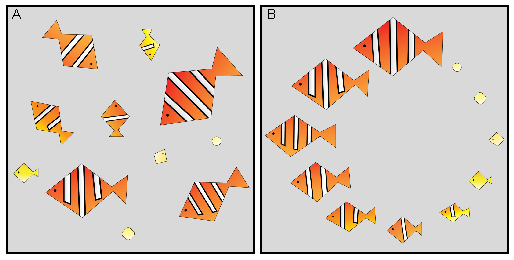
\includegraphics{fig1}
\caption{Caricature illustrating the tasks of image registration and temporal ordering. {\xfigtextfontit (A)} Images of ``samples'', each in a different orientation and a different stage of development. {\xfigtextfontit (B)} Registered and ordered samples. For this caricature, the registration and ordering is straightforward because the data set is small, the landmarks are visually apparent, and the developmental changes are easy to recognize.}
%\label{fig:fish}
\customlabel{fig:fish}{1}
\customlabel{subfig:fish_unordered}{\ref{fig:fish}{\it A}}
\customlabel{subfig:fish_ordered}{\ref{fig:fish}{\it B}}
\end{figure}


We describe an algorithmic approach to registration and temporal ordering that is robust to these sources of error.
%
In contrast to a number of previous approaches, it does not rely on the {\em a priori} knowledge of spatial landmarks and markers of developmental progression that can be used to align and order images \cite{zitova2003image, rowley1998rotation, hajnal2010medical, greenspan1994rotation, zhao2003face}.
%
It is based on a manifold learning algorithm (vector diffusion maps, VDM \cite{singer2012vector}) which simultaneously addresses the problems of registration and temporal ordering. 
%
This algorithm is one of several nonlinear dimensionality reduction techniques that have been developed over the past decade \cite{Belkin2003, coifman2005geometric, coifman2006geometric, tenenbaum2000global, roweis2000nonlinear}, with
applications ranging from analysis of cryo-electron microscopy (cryo-EM) images of individual molecules  \cite{zhao2014rotationally, singer2011viewing} to face recognition \cite{lafon2006data}.
%
Here, the vector diffusion maps algorithm is adapted for the analysis of images of developing embryos from cross-sectional studies of developmental dynamics, with the main objective of revealing stereotypic developmental trajectories.
%
To illustrate our approach, we analyze two data sets from a study of {\it Drosophila} embryogenesis, one of the best experimental models for studies of developmental dynamics \cite{jaeger2012drosophila}.
%
Our first data set, from a live imaging study where the correct rotational orientation and temporal order are independently known, will be used to validate our approach.
%
The correct orientation and order is unknown for the second data set comprised of images from fixed embryos; here, we will show how the algorithm can help uncover developmental dynamics which are not readily apparent. 


\section{Results}

\subsection{Vector diffusion maps for registration and temporal ordering}

Vector diffusion maps \cite{singer2012vector} is a manifold learning
technique developed for data sets which contain two types of sources of variability:
geometric symmetries (such as rotations of the images) which one would like to factor out,
and ``additional" directions of variability (such as temporal dynamics) which one would like to uncover.
%
Vector diffusion maps combine two algorithms, {\em angular synchronization} \cite{singer2011angular} for image registration and {\em diffusion maps} \cite{coifman2005geometric} for extracting intrinsic low-dimensional structure in data, into a single computation.
%
We will use the algorithm to register images of developing embryos with respect to rotations, as well as uncover the main direction of variability {\it after} removing rotational symmetries.
%
We assume that the main direction of variability in these images is parameterized by the developmental time of each embryo.
%
As a consequence, uncovering this direction will allow us to recover the developmental dynamics.

Angular synchronization uses pairwise alignment information to register a set of images in a globally consistent way.
%
A schematic illustration of angular synchronization is shown in \fig~\ref{subfig:synch1}, where each image is represented as a vector, and the goal is to align the set of vectors.
%
We first compute the angles needed to align pairs of vectors (or images).  
%
In general, this requires no template function \cite{ahuja2007template} or image landmarks \cite{ian1998statistical}.
%
Using the alignment angles between all pairs of vectors, angular synchronization finds the set of rotation angles (one angle for each vector) that is most consistent with {\it all} pairwise measurements (see \SI); this is illustrated in \fig~\ref{subfig:synch2}.
%
In this schematic, registration via angular synchronization is trivial, as the pairwise measurements contain no noise.
%
However, the algorithm can successfully register data sets even when many of the pairwise measurements are inaccurate \cite{singer2011angular}.


After removing variability due to rotations, the developmental dynamics may be revealed by ordering the data along the one-dimensional manifold that parameterizes most of the remaining variability in the data.
%
Such a manifold can be discovered using diffusion maps \cite{coifman2005geometric}, a nonlinear dimensionality reduction technique that uncovers an intrinsic parametrization of data that lies on a low-dimensional, perhaps nonlinear, manifold in high-dimensional space.
%
The idea is illustrated in \fig~\ref{subfig:dmaps1}, where the data are two-dimensional points which lie on a one-dimensional nonlinear curve.
%
We use {\it local} information about the data to find a parametrization  which respects the underlying manifold geometry, so that points which are close in high-dimensional space (e.g., images which look similar) are close in our parametrization.
%
This idea of locality is denoted by the edges in \fig~\ref{subfig:dmaps1}.
%
Data points which are close are connected by dark edges, and clearly, the dark edges are more ``informative" about the low-dimensional structure of the data.
%
The color in \fig~\ref{subfig:dmaps2} depicts the one-dimensional parametrization or ordering of the data that we can detect visually.
%
In our working examples, each data point will be of much higher dimension (e.g., a pixelated image), and so we cannot extract this low-dimensional structure visually.
%
Instead, we will use diffusion maps to automatically uncover a parametrization of our high-dimensional data (see \SI).
%
Diffusion maps generalizes directly from one-dimensional nonlinear curves to higher-dimensional manifolds.

\begin{figure}[t]
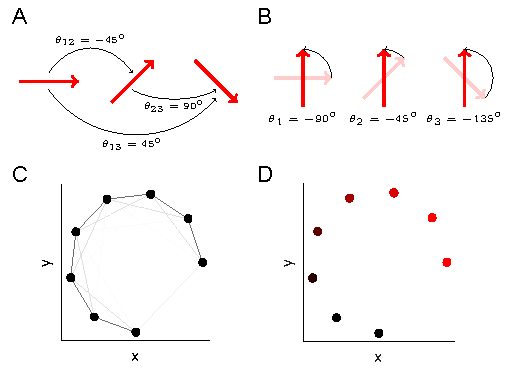
\includegraphics{fig2}
\caption{Schematic illustrating angular synchronization and diffusion maps. {\xfigtextfontit (A)} Set of vectors, each in a different orientation. The pairwise alignment angles are indicated. {\xfigtextfontit (B)} The vectors from {\xfigtextfontit A}, each rotated about their midpoint so that the set is globally aligned. Note that the chosen rotation angles are consistent with the pairwise alignments in {\xfigtextfontit A}: the differences between a pair of angles in {\xfigtextfontit B} is the same as the pairwise angle in {\xfigtextfontit A}. {\xfigtextfontit (C)} Data points (in black) which lie on a one-dimensional nonlinear curve in two dimensions. Each pair of points is connected by an edge, and the edge weight is related to the Euclidean distance between the points through the diffusion kernel (see {\xfigtextfontit \SI}), so that close data points are connected by darker (``stronger'') edges. {\xfigtextfontit (D)} The data in {\xfigtextfontit C}, colored by the first (non-trivial) eigenvector from the diffusion map computational procedure. The color intensity is monotonic with the perceived curve arclength, thus parameterizing the curve.}
%\label{fig:schematics}
\customlabel{fig:schematics}{2}
\customlabel{subfig:synch1}{\ref{fig:schematics}{\it A}}
\customlabel{subfig:synch2}{\ref{fig:schematics}{\it B}}
\customlabel{subfig:dmaps1}{\ref{fig:schematics}{\it C}}
\customlabel{subfig:dmaps2}{\ref{fig:schematics}{\it D}}
\end{figure}

\begin{figure*}[t]
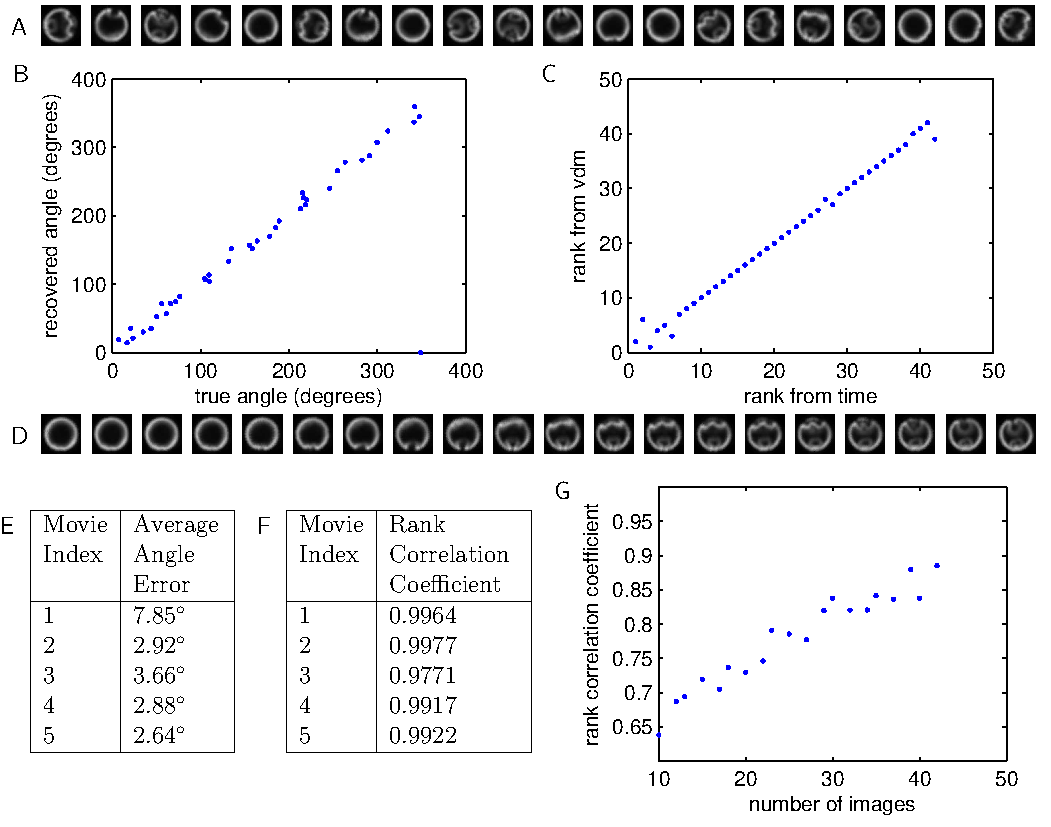
\includegraphics{fig3}
\caption{Method validation using live imaging of {\xfigtextfontit Drosophila} embryos.{\xfigtextfontit (A)} Selected images from a live imaging study of a {\xfigtextfontit Drosophilla} embryo during gastrulation. Each frame is in an arbitrary rotational orientation, and the order of the frames has been shuffled. {\xfigtextfontit (B)} Images from {\xfigtextfontit A} after registration and ordering using vector diffusion maps. The dorsal side of each embryo now appears at the top of each image, and the ventral side appears at the bottom. {\xfigtextfontit (C)} The correlation between the recovered rotation angle (using vector diffusion maps) and the true rotation angle for each frame in the movie. {\xfigtextfontit (D)} The correlation between the recovered rank (using vector diffusion maps) and the true rank for each frame in the movie. {\xfigtextfontit (E)} The average error in the recovered angle and the rank correlation coefficient for $5$ different movies. {\xfigtextfontit (F)} The median rank correlation coefficient (over $200$ samples) as a function of the number of images in the data set. }
\customlabel{fig:movie}{3}
\customlabel{subfig:movie_unregistered_unordered}{\ref{fig:movie}{\it A}}
\customlabel{subfig:movie_registered_ordered}{\ref{fig:movie}{\it B}}
\customlabel{subfig:movie_angle_corr}{\ref{fig:movie}{\it C}}
\customlabel{subfig:movie_rank_corr}{\ref{fig:movie}{\it D}}
\customlabel{subfig:movie_error_table}{\ref{fig:movie}{\it E}}
\customlabel{subfig:movie_bootstrap}{\ref{fig:movie}{\it F}}
\end{figure*}


\subsection{Method validation using live imaging}

To validate the proposed approach, we applied our algorithm to a dataset where the true temporal order and rotational orientation of the images are known {\em a priori}.
%
This data set was obtained through live imaging of a single {\it Drosophila} embryo during the twenty minutes spanning late stages of cellularization through early gastrulation.
%
During this time window, the ventral furrow is formed, where the ventral side buckles towards the center of the embryo, internalizing the future muscle cells, eventually forming a characteristic ``omega'' shape.
%
Germband extension then causes cells from the ventral side to move towards the posterior pole of the embryo, and then wrap around to the dorsal side \cite{leptin2005gastrulation}.
%
At the end of this process, cells which were originally on the ventral and posterior side of the embryo find themselves on the dorsal side, causing a similar ``omega'' to appear on the dorsal side.

\fig~\ref{subfig:movie_unregistered_unordered} shows selected images from this live imaging study. 
%
The entire data set contains $40$ consecutive frames taken at $30$~second time intervals.
%
Each image shows an optical cross-section at a fixed depth of a vertically oriented developing embryo, with the nuclei labeled by Histone-GFP.
%
Each frame was arbitrarily rotated, and the order of the frames was scrambled.
%
The task is now to register these images and order them in time to reconstruct the developmental trajectory.

We used vector diffusion maps to register and order the images. 
%
\fig~\ref{subfig:movie_registered_ordered} shows the images from \fig~\ref{subfig:movie_unregistered_unordered}, now registered and ordered; the real time for each frame is also indicated.
%
With a small number of exceptions, the recovered ordering is consistent with the real time dynamics. 
%
\fig~\ref{subfig:movie_angle_corr} and \fig~\ref{subfig:movie_rank_corr}  show the correlations between the recovered and true angles and ranks, respectively, for the entire data set. 
%
Both the angles and the ranks are recovered with a high degree of accuracy.

To assess the robustness of our proposed methodology, we repeated this procedure with four additional datasets extracted from independent live imaging studies spanning the same developmental time period. 
%
The results are shown in \fig~\ref{subfig:movie_error_table}. 
%
The errors in the recovered angles are all less than 10$^\circ$, and the rank correlation coefficients are consistently greater than $0.95$, indicating that our methodology can reproducibly order data of this type. 

In general, to accurately recover the temporal order, the vector diffusion maps algorithm requires a sufficient amount of data so that the underlying one-dimensional curve (i.e., the curve in \fig~\ref{subfig:dmaps1}) is well-sampled;
the accuracy of the recovered alignments is a function of the signal-to-noise ratio in the pairwise alignments, as well as the size of the data set \cite{singer2011angular}.
%
Clearly, $40$ images are sufficient to accurately recover the rotational orientation and temporal order  in this specific developmental time frame.
%
To quantitatively assess how our methods perform as a function of sample size, we used bootstrap sampling to compute the rank correlation as a function of the size of the data set.
%
\fig~\ref{subfig:movie_bootstrap} shows the median rank correlation coefficient as a function of the number of images, where each point is the average over $200$ bootstrap samples.
%
As expected, the accuracy in the recovered ordering increases with the number of images. 
%
The errors in the recovered angles did not vary significantly with the number of images and were consistently less than $10^{\circ}$;
because our particular data set contains relatively low noise levels, few images are required to obtain accurate rotational alignments. 
%
We have therefore demonstrated that the algorithm accurately registers and orders a model data set where both the rotation angles and real times are independently known. 
%
We also demonstrated that these results are consistent across multiple data sets, and showed how the accuracy of our methods varies as a function of the number of images.


\subsection{Datasets with interembryo variability}

Arguably, the most common source of noise within developmental biology experiments is embryo-to-embryo variability. 
%
We would like to demonstrate that our methods are robust to such noise sources. 
%
We constructed synthetic time course data sets by selecting a frame from a random live imaging experiment for each time point, and used our methodology to register and order these sets. 
% 
The median rank correlation coefficient for these synthetic time courses was found to be 0.81, indicating that our methodology can still accurately recover the temporal order even under noisy conditions. 

Because live imaging data represents only a small fraction of the data collected in developmental biology experiments, the utility of our proposed methodology is in the analysis of large data sets of fixed images, where the developmental times and spatial orientations are unknown. 
%
To demonstrate such an application, \fig~\ref{subfig:fixed_images_unregistered_unordered} shows selected images from a set of $120$ images (see \SI  for the full data set) which cover a thirty minute time interval spanning late cellularization through gastrulation.
%
This data set is more complex than the live imaging data sets in that it contains many more images, each with several channels.
%
Each image is an optical cross-section of a {\em different} vertically oriented embryo fixed at a different (and unknown) developmental time.
%
The nuclei (gray) were labeled with DAPI, a DNA stain.
%
Embryos were stained with the antibody that recognizes Twist (Twi, shown in green), a transcription factor which specifies the cells of the future muscle tissue.
%
Another signal is provided by the phosphorylated form of the extracellular signal regulated kinase (dpERK, shown in red), an enzyme that, in this context, specifies a subset of neuronal cells.

\begin{figure*}[t]
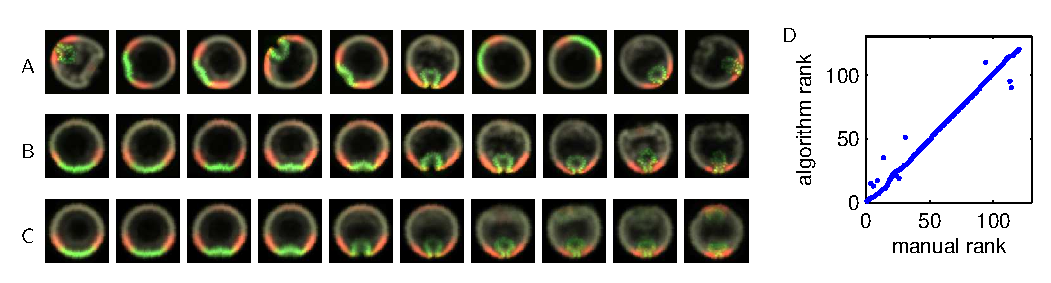
\includegraphics{fig4}
\caption{Fixed {\xfigtextfontit Drosophila} embryos during gastrulation. {\xfigtextfontit (A)} Images of gastrulating embryos, stained for nuclei (gray), Twi (green), and dpERK (red). Each image is of a different embryo arrested at a different developmental time and in a different rotational orientation. {\xfigtextfontit (B)} Data from {\xfigtextfontit A}, registered and ordered using vector diffusion maps. The expert rank for each image is indicated. {\xfigtextfontit (C)} A representative ``developmental trajectory'' obtained from local averaging of the entire set of registered and ordered images (see \SI). {\xfigtextfontit (D)} Correlation between the image ranks calculated from the vector diffusion maps algorithm and the ranks obtained from ordering by an expert. The rank correlation coefficient is $0.97$. }
\customlabel{fig:data2}{4}
\customlabel{subfig:fixed_images_unregistered_unordered}{\ref{fig:data2}{\it A}}
\customlabel{subfig:fixed_images_registered_ordered}{\ref{fig:data2}{\it B}}
\customlabel{subfig:fixed_images_average_trajectory}{\ref{fig:data2}{\it C}}
\customlabel{subfig:fixed_images_rank_corr}{\ref{fig:data2}{\it D}}
\end{figure*}

\fig~\ref{subfig:fixed_images_registered_ordered} shows the images from \fig~\ref{subfig:fixed_images_unregistered_unordered}, now registered and ordered using vector diffusion maps \cite{singer2012vector}.
%
However, because of interembryo variability, the selected images are not entirely representative of the developmental dynamics across the entire data set.
%
To highlight the developmental dynamics revealed by vector diffusion maps, we computed an average developmental trajectory across the set of registered and ordered images (see \SI). 
%
Sequential snapshots of this averaged trajectory, shown in \fig~\ref{subfig:fixed_images_average_trajectory}, serve as a summary of the stereotypic developmental dynamics.
%
We can now easily see the developmental progression, which is consistent with known dynamics. 
%
dpERK first appears as two lateral peaks at the ventral side of the embryo; a third dpERK peak then appears at the dorsal side of the embryo.
%
During invagination, the two ventral dpERK peaks merge together, eventually forming (together with Twi) the ``omega'' shape.
%
The dorsal dpERK peak then disappears during germband extension as cells from the ventral side wrap around to the dorsal side.
%
At the end of this process, similar ``omega'' shaped patterns formed by Twi and dpERK appear on the dorsal side; these patterns are most readily seen in the last image of \fig~\ref{subfig:fixed_images_average_trajectory}.
%
Thus, vector diffusion maps can accomplish the tasks presented in the caricature in \fig~\ref{fig:fish}, even in the absence of information about image landmarks (e.g., fins) and without {\it a priori} knowledge of developmental dynamics (e.g., correlation of age with body size).

To evaluate the quality of our registration and ordering, we can use prior knowledge about the developmental dynamics. 
%
The Twi signal is known to form a Gaussian peak at the ventralmost point of the embryo. 
%
TODO: add more...
%
Because the developmental time of each embryo cannot be easily estimated, we have few options for evaluating the quality of our ordering. 
%
We compared the ordering obtained from vector diffusion maps to an expert ordering provided by a trained embryologist who is knowledgeable about the developmental progression and the important image features.  
%
The results (see \fig~\ref{subfig:fixed_images_rank_corr}) show that our ordering is consistent with the expert ordering. 
%
However, manually ordering the images is nontrivial for researchers who are not familiar with the developmental progression, and can be tedious and time-consuming for those who are.
%
In contrast, our method requires relatively little computational time, taking $15$~seconds on an Intel Core i7 2.93 GHz processor. %for $100$ images of $100 \times 100$ pixels, using 10$^{\circ}$ rotational discretizations.
%
Empirically, we found the CPU time required was $\mathcal{O}(n)$ in the number of pixels and the number of rotations, and $\mathcal{O}(n^{1.5})$ in the number of images in the data set.
%
Furthermore, the computation of the pairwise rotational alignments, which is the most computationally intensive portion of the calculation, is trivially parallelizable.
%
The requisite human intervention and tuning for our method is relatively small. 
%
Images must first be minimally preprocessed so that the Euclidean distance between the pixels in informative. 
%
%The image resolution should be chosen as low as possible while still retaining the important image features, as the computational cost increases with the number of pixels.
%
The two algorithmic parameters are the number of discretization points required to compute the pairwise alignments, and the kernel scale.
%
In our examples, we use 10$^{\circ}$ angle discretizations for the pairwise alignments, and one-tenth of the median pairwise distance for the kernel scale. 
%
We found that the results are robust to both of these parameters% (5$^{\circ}$--30$^{\circ}$ angle discretizations and kernel scales of one-fifth to one-twentieth of the median pairwise distances all yielded acceptable results)
, and that these parameter values were appropriate for all of the data sets presented in this paper. 
%
Image preprocessing and selecting these two parameters are relatively simple tasks compared to manual registration and ordering of images, especially when the data sets are large.  
%
Therefore, this methodology is very promising for much larger imaging data sets which are impractical to evaluate manually. 


\section{Discussion}

We presented a unified approach to temporal ordering and registration of images in studies of developmental dynamics. 
%
To the best of our knowledge, algorithmic approaches to these two tasks have been explored largely independently of each other. 
%
In particular, temporal ordering of imaging data sets was done with a significant amount of human supervision and using registered images as a starting point \cite{yuan2014automated, surkova2008characterization}.  
%
In parallel, ordering of large-scale cross-sectional data was done in the context of molecular profiling studies, in which data are vectors describing the amounts of different chemical species \cite{anavy2014blind, trapnell2014dynamics, gupta2008extracting}. 
%
Automated temporal ordering of such data sets was accomplished by first projecting the data onto a low-dimensional subspace spanned by the leading principal or independent components, and then solving a traveling salesman problem or constructing a minimum spanning tree on the projected data to order multiple snapshots. 
%
The presented approach addresses image registration and ordering in a single step and orders the data without first projecting them on a low-dimensional subspace.
%; vector diffusion maps can also order images when global registration of the entire data set is topologically impossible \cite{zhao2014rotationally}.
%
%The task of image registration has been widely studied \cite{zitova2003image}, for applications such as face recognition \cite{rowley1998rotation}, medical image registration \cite{hajnal2010medical}, and texture classification \cite{greenspan1994rotation}.
%
In contrast to most of the existing approaches to image registration which rely on the knowledge about some landmarks in the data \cite{ian1998statistical} (such as the eyes in face recognition applications \cite{zhao2003face}), algorithms based on angular synchronization can register images even in the absence of such information, making them applicable to a wide variety of applications. 
%
Although we have presented results for a specific type of data (images along the dorsoventral axis of developing {\em Drosophila} embryos), because the methodology only relies on computing distances between images, we are confident that they can be readily applied and extended to many other imaging data sets. 

Previously, angular synchronization and vector diffusion maps have been used to reconstruct molecular shapes from cryo-electron microscopy images \cite{singer2012vector, zhao2014rotationally, singer2011viewing}.
%
Because of high levels of instrument noise in these data, thousands of images were needed for successful shape reconstruction. 
%
Based on the presented results, we expect that much smaller data sets may be sufficient for successful reconstruction of developmental trajectories.
%
In general, the size of the data set required is a function of the instrument noise, interembryo variablity, and the complexity of the developmental dynamics.
%
%Here, we have used vector diffusion maps to register the images with respect to rotations; however, one could factor out other sources of variability, such as translations, reflections \cite{singer2012vector, goemans1995improved, bandeira2013cheeger} or dilations.
 
As experimental imaging becomes faster and less expensive, the rate of collection of imaging data will surpass the rate of manual image analysis,
and we will require automated methodologies which are sufficiently general to address a wide variety of applications to organize such large data sets.
%
Vector diffusion maps allows us to automatically register images, an essential task for many applications.
%
Simultaneously, the algorithm provides us with coordinates for each image.
%
In the examples presented here, we have focused on recovering a single coordinate which is used to order the images in time.
%
In general, we can recover several coordinates that are good descriptors of our data set.
%
This parameterization can then be used for typical data analysis tasks, such as outlier detection, clustering, and model fitting. 
%
Images taken from different viewing directions can be analyzed, as the vector diffusion maps parameterization will organize the images according to the viewing angle.
%
Another direction for future work is related to the joint analysis of data sets provided by different imaging approaches, such as merging live imaging data of tissue morphogenesis with snapshots of cell signaling and gene expression from fixed embryos \cite{krzic2012multiview, ichikawa2014live, rubel2010coupling}.  
%
Given the rapidly increasing volumes of imaging data from studies of multiple developmental systems, we expect that dimensionality reduction approaches discussed in this work will be increasingly useful for biologists and motivate future applications and algorithmic advances. 
  

%% == end of paper:

%% Optional Materials and Methods Section
%% The Materials and Methods section header will be added automatically.

%% Enter any subheads and the Materials and Methods text below.


\begin{materials}

\section{Fly strain and whole-mount immunostaining}
%
Oregon-R (OreR) and spaghetti squash (Sqh)-GFP were used as wild type strains. 
%
{\it Sna\textsuperscript{\it IIG05}/Cyo hb-lacZ} flies were used to study mutant embryos with one peak of dpERK activation.  
%
Embryos were collected and fixed at 22$^\circ$C. 
%
Monoclonal rabbit anti-dpERK (1:100, Cell signaling), mouse anti-Dorsal (1:100, Developmental Studies Hybridoma Bank), rat anti-Twist (1:500, a gift from Eric Wieschaus), and mouse anti-beta-galactosidase (1:500, DSHB) were used to stain proteins of interest. DAPI (1:10,000, Vector Laboratories) was used to visualize nuclei, and Alexa Fluors (1:500, Invitrogen) were used as secondary antibodies. 

\section{Microscopy}
%
Nikon A1-RS scanning confocal microscope, and the Nikon 60X Plan-Apo oil objective was used to image embryos. Embryos were collected, stained, and imaged together under the same microscope setting. End-on imaging was performed by using the microfluidics device described previously. Images were collected at the focal plane $\sim$90~$\mathrm{\mu m}$ from the posterior pole of an embryo (see \fig~\ref{fig:DV_view}). 

\section{Image preprocessing}
%
Borders were cropped from each image using a Canny edge-detection filter to remove any size effects.
%
Adaptive histogram equalization was used to normalize the nuclear signal intensity throughout each image, and a 5-pixel radius disk filter was used to smooth the nuclear signal. 
%
%For the three-channel fixed images, the nuclear signal was scaled by half relative to the Twi and dpERK signals.

\section{Software}
%
The vector diffusion maps algorithms was implemented in MATLAB\textsuperscript{\textregistered} (R2013b, The MathWorks, Natick, Massachusetts).
%
All code, including all the scripts used to generate the figures in this paper, is available at .....

\end{materials}


%% Optional Appendix or Appendices
%% \appendix Appendix text...
%% or, for appendix with title, use square brackets:
%% \appendix[Appendix Title]


\begin{acknowledgments}
The authors thank Adam Finkelstein,  Thomas Funkhouser, and John Storey for helpful discussions. 
%
C.J.D. was supported by the Department of Energy Computational Science Graduate Fellowship (CSGF), grant number DE-FG02-97ER25308.
%
B.L. and S.Y.S. were supported by the National Institutes of Health Grant R01GM086537. 
%
T.J.L. and H.L. were supported by the National Science Foundation Grant Emerging Frontiers in Research and Innovation (EFRI) 1136913.
%
A.S. was supported by the Air Force Office of Scientific Research Grant
FA9550-12-1-0317.
%
I.G.K. was supported by the National Science Foundation (CS\&E program).
\end{acknowledgments}

%% PNAS does not support submission of supporting .tex files such as BibTeX.
%% Instead all references must be included in the article .tex document.
%% If you currently use BibTeX, your bibliography is formed because the
%% command \verb+\bibliography{}+ brings the <filename>.bbl file into your
%% .tex document. To conform to PNAS requirements, copy the reference listings
%% from your .bbl file and add them to the article .tex file, using the
%% bibliography environment described above.

%%  Contact pnas@nas.edu if you need assistance with your
%%  bibliography.

% Sample bibliography item in PNAS format:
%% \bibitem{in-text reference} comma-separated author names up to 5,
%% for more than 5 authors use first author last name et al. (year published)
%% article title  {\it Journal Name} volume #: start page-end page.
%% ie,
% \bibitem{Neuhaus} Neuhaus J-M, Sitcher L, Meins F, Jr, Boller T (1991)
% A short C-terminal sequence is necessary and sufficient for the
% targeting of chitinases to the plant vacuole.
% {\it Proc Natl Acad Sci USA} 88:10362-10366.


%% Enter the largest bibliography number in the facing curly brackets
%% following \begin{thebibliography}

\bibliographystyle{pnas2}
\bibliography{../image_analysis_paper/background_reading/references,../../references/references}

\end{article}

\end{document}




